% answers.tex —— 2008 年·普通高等学校招生考试·浙江卷·理科 · 参考答案与详细解析片段
% 由 tools/generate_projects.py 依来源总账自 2008/2008_数学真题_浙江理_试题.md + 2008/2008_数学真题_浙江理_解析正文.md + 2008/2008_数学真题_浙江理_答案要点.md 生成，勿手改（改源 MD 后重跑）


\begin{gktip}
固定候选 PDF 仅含题面，无答案、解析和评分标准，原卷亦未标注分值；以下为非官方编者独立推导，官方答案字段为空。来源发布者、出版者、版次与官方身份均未核。
\end{gktip}

\begin{answer}
\gksolhead{1}{}

\textbf{题目}：

已知 $a$ 是实数，$\dfrac{a-\mathrm i}{1+\mathrm i}$ 是纯虚数，则 $a=$（　）

（A）$1$

（B）$-1$

（C）$\sqrt2$

（D）$-\sqrt2$

\Needspace{4\baselineskip}
\textbf{解析}

\Needspace{5\baselineskip}
计算如下：

\nopagebreak[4]
\[\frac{a-\mathrm i}{1+\mathrm i}=\frac{(a-\mathrm i)(1-\mathrm i)}2=\frac{a-1}2-\frac{a+1}2\mathrm i,\]

纯虚数要求实部为零，故 $a=1$（此时虚部 $-1\neq0$）。

\gkanswer{答案：A。}

\end{answer}
\begin{answer}
\gksolhead{2}{}

\textbf{题目}：

已知 $U=\mathbf R$，$A=\{x\mid x>0\}$，$B=\{x\mid x\leqslant-1\}$，则 $\left(A\cap\complement_UB\right)\cup\left(B\cap\complement_UA\right)=$（　）

（A）$\varnothing$

（B）$\{x\mid x\leqslant0\}$

（C）$\{x\mid x>-1\}$

（D）$\{x\mid x>0\text{ \text{或} }x\leqslant-1\}$

\Needspace{4\baselineskip}
\textbf{解析}

\Needspace{5\baselineskip}
$A$ 与 $B$ 不相交，$\left(A\cap\complement_UB\right)\cup\left(B\cap\complement_UA\right)=A\cup B$，即

\nopagebreak[4]
\[\{x\mid x>0\text{ \text{或} }x\leqslant-1\}.\]

\gkanswer{答案：D。}

\end{answer}
\begin{answer}
\gksolhead{3}{}

\textbf{题目}：

已知 $a$，$b$ 都是实数，那么“$a^2>b^2$”是“$a>b$”的（　）

（A）充分而不必要条件

（B）必要而不充分条件

（C）充分必要条件

（D）既不充分也不必要条件

\Needspace{4\baselineskip}
\textbf{解析}

$a^2>b^2$ 即 $|a|>|b|$。取 $a=-2$，$b=1$ 与 $a=1$，$b=-2$ 分别否定充分性与必要性。

\gkanswer{答案：D。}

\end{answer}
\begin{answer}
\gksolhead{4}{}

\textbf{题目}：

在 $(x-1)(x-2)(x-3)(x-4)(x-5)$ 的展开式中，含 $x^4$ 的项的系数是（　）

（A）$-15$

（B）$85$

（C）$-120$

（D）$274$

\Needspace{4\baselineskip}
\textbf{解析}

五个因式中取四个的 $x$、余下一个取常数，故 $x^4$ 的系数为 $-(1+2+3+4+5)=-15$。

\gkanswer{答案：A。}

\end{answer}
\begin{answer}
\gksolhead{5}{}

\textbf{题目}：

在同一平面直角坐标系中，函数 $y=\cos\left(\dfrac x2+\dfrac{3\pi}2\right)$（$x\in[0,2\pi]$）的图象和直线 $y=\dfrac12$ 的交点个数是（　）

（A）$0$

（B）$1$

（C）$2$

（D）$4$

\Needspace{4\baselineskip}
\textbf{解析}

\Needspace{5\baselineskip}
计算如下：

\nopagebreak[4]
\[\cos\left(\frac x2+\frac{3\pi}2\right)=\sin\frac x2,\]

$x\in[0,2\pi]$ 时 $\dfrac x2\in[0,\pi]$，$\sin\dfrac x2=\dfrac12$ 有两解。

\gkanswer{答案：C。}

\end{answer}
\begin{answer}
\gksolhead{6}{}

\textbf{题目}：

已知 $\{a_n\}$ 是等比数列，$a_2=2$，$a_5=\dfrac14$，则 $a_1a_2+a_2a_3+\cdots+a_na_{n+1}=$（　）

（A）$16\left(1-4^{-n}\right)$

（B）$16\left(1-2^{-n}\right)$

（C）$\dfrac{32}3\left(1-4^{-n}\right)$

（D）$\dfrac{32}3\left(1-2^{-n}\right)$

\Needspace{4\baselineskip}
\textbf{解析}

\Needspace{5\baselineskip}
$a_1=\dfrac{a_2}{q}$，由 $a_5=a_2q^3$ 得 $q^3=\dfrac18$，$q=\dfrac12$，$a_1=4$。故 $\{a_na_{n+1}\}$ 是首项 $a_1a_2=8$、公比 $q^2=\dfrac14$ 的等比数列，

\nopagebreak[4]
\[\sum_{k=1}^na_ka_{k+1}=\frac{8\left(1-4^{-n}\right)}{1-\frac14}=\frac{32}3\left(1-4^{-n}\right).\]

\gkanswer{答案：C。}

\end{answer}
\begin{answer}
\gksolhead{7}{}

\textbf{题目}：

若双曲线 $\dfrac{x^2}{a^2}-\dfrac{y^2}{b^2}=1$ 的两个焦点到一条准线的距离之比为 $3:2$，则双曲线的离心率是（　）

（A）$3$

（B）$5$

（C）$\sqrt3$

（D）$\sqrt5$

\Needspace{4\baselineskip}
\textbf{解析}

\Needspace{5\baselineskip}
取右准线 $x=\dfrac{a^2}c$，两焦点到它的距离分别为 $c-\dfrac{a^2}c$ 与 $c+\dfrac{a^2}c$，

\nopagebreak[4]
\[\frac{c+\frac{a^2}c}{c-\frac{a^2}c}=\frac32\ \Longrightarrow\ c^2=5a^2\ \Longrightarrow\ e=\sqrt5.\]

\gkanswer{答案：D。}

\end{answer}
\begin{answer}
\gksolhead{8}{}

\textbf{题目}：

若 $\cos\alpha+2\sin\alpha=-\sqrt5$，则 $\tan\alpha=$（　）

（A）$\dfrac12$

（B）$2$

（C）$-\dfrac12$

（D）$-2$

\Needspace{4\baselineskip}
\textbf{解析}

\Needspace{5\baselineskip}
$\cos\alpha+2\sin\alpha=\sqrt5\cos(\alpha-\varphi)$（其中 $\cos\varphi=\dfrac1{\sqrt5}$，$\sin\varphi=\dfrac2{\sqrt5}$），最小值为 $-\sqrt5$，故取到最小值时

\nopagebreak[4]
\[\cos\alpha=-\frac1{\sqrt5},\qquad \sin\alpha=-\frac2{\sqrt5},\qquad \tan\alpha=2.\]

\gkanswer{答案：B。}

\end{answer}
\begin{answer}
\gksolhead{9}{}

\textbf{题目}：

已知 $\boldsymbol a$，$\boldsymbol b$ 是平面内两个互相垂直的单位向量，若向量 $\boldsymbol c$ 满足 $(\boldsymbol a-\boldsymbol c)\cdot(\boldsymbol b-\boldsymbol c)=0$，则 $|\boldsymbol c|$ 的最大值是（　）

（A）$1$

（B）$2$

（C）$\sqrt2$

（D）$\dfrac{\sqrt2}2$

\Needspace{4\baselineskip}
\textbf{解析}

\Needspace{5\baselineskip}
取 $\boldsymbol a=(1,0)$，$\boldsymbol b=(0,1)$，$\boldsymbol c=(x,y)$，条件即

\nopagebreak[4]
\[x^2+y^2=x+y\ \Longleftrightarrow\ \left(x-\frac12\right)^2+\left(y-\frac12\right)^2=\frac12,\]

\Needspace{5\baselineskip}
故 $|\boldsymbol c|$ 的最大值为圆心到原点的距离加半径：

\nopagebreak[4]
\[\frac{\sqrt2}2+\frac{\sqrt2}2=\sqrt2.\]

\gkanswer{答案：C。}

\end{answer}
\begin{answer}
\gksolhead{10}{}

\textbf{题目}：

如图，$AB$ 是平面 $\alpha$ 的斜线段，$A$ 为斜足。若点 $P$ 在平面 $\alpha$ 内运动，使得 $\triangle ABP$ 的面积为定值，则动点 $P$ 的轨迹是（　）
\nopagebreak[4]
\begin{center}% 2008 年浙江卷理科第 10 题：AB 是平面 α 的斜线段，A 为斜足，P 在平面 α 内运动，
%   使 △ABP 的面积为定值。
% 来源 PDF：gaokaomath-src/普通高考/2008/2008浙江理.pdf
% SHA-256：61b86d188443ba25020577365e293aa0999ec32fb32b9791690cec6ac85cf0db
% 原页：2008浙江理.pdf 第 1 页（A3 三栏）第 1 栏，书页码 491。
% 重绘依据：平面 α 画成平行四边形，B 在平面上方，A 为平面内的斜足（与 B 的射影 H 分开），
%   P 在平面内右侧；BA、BP、AP 实线，B 到平面的垂线 BH 为虚线。
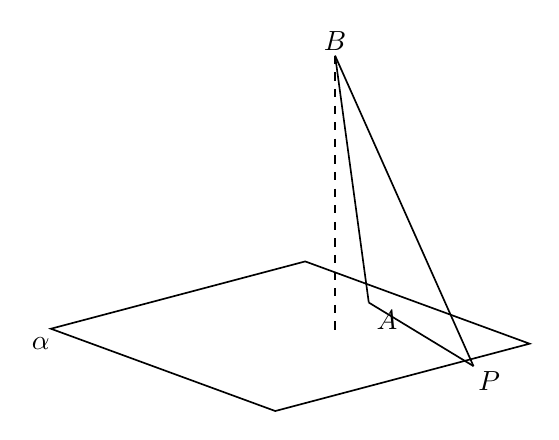
\begin{tikzpicture}[scale=0.95, semithick, every node/.style={inner sep=1.5pt}]
  % 平面 α
  \draw (-2.2,-0.45) -- (0.8,-1.55) -- (4.2,-0.65) -- (1.2,0.45) -- cycle;
  \node[below left] at (-2.15,-0.5) {$\alpha$};

  \coordinate (B) at (1.60,3.20);
  \coordinate (H) at (1.60,-0.55);
  \coordinate (A) at (2.05,-0.10);
  \coordinate (P) at (3.45,-0.95);

  \draw (B) -- (A);
  \draw (B) -- (P);
  \draw (A) -- (P);
  \draw[dashed] (B) -- (H);

  \node[above] at (B) {$B$};
  \node[below right=1pt] at (A) {$A$};
  \node[below right] at (P) {$P$};
\end{tikzpicture}
\end{center}
\nopagebreak[4]
（A）圆

（B）椭圆

（C）一条直线

（D）两条平行直线

\Needspace{4\baselineskip}
\textbf{解析}

设 $AB$ 与平面 $\alpha$ 所成角为 $\theta$，$A$ 为斜足，$B$ 在 $\alpha$ 上的射影为 $B'$，$AB'=AB\cos\theta$。对 $P\in\alpha$，$\triangle ABP$ 的面积为定值等价于 $P$ 到直线 $AB$ 的距离为定值 $d$。

\Needspace{5\baselineskip}
以 $A$ 为原点、$AB'$ 为 $x$ 轴建立坐标系，设 $P(x,y)$，则 $P$ 到直线 $AB$（方向 $(\cos\theta,0,\sin\theta)$）的距离满足

\nopagebreak[4]
\[d^2=x^2\sin^2\theta+y^2,\]

这是椭圆（$\theta\neq0$）。

\gkanswer{答案：B。}

\end{answer}
\begin{answer}
\gksolhead{11}{}

\textbf{题目}：

已知 $a>0$，若平面内三点 $A(1,-a)$，$B(2,a^2)$，$C(3,a^3)$ 共线，则 $a=$\gkblank{}。

\Needspace{4\baselineskip}
\textbf{解析}

\Needspace{5\baselineskip}
三点共线给

\nopagebreak[4]
\[\frac{a^2+a}{2-1}=\frac{a^3+a}{3-1}\ \Longrightarrow\ a^3-2a^2-a=0\ \Longrightarrow\ a\left(a^2-2a-1\right)=0.\]

由 $a>0$ 得 $a=1+\sqrt2$。

\gkanswer{答案：$1+\sqrt2$。}

\end{answer}
\begin{answer}
\gksolhead{12}{}

\textbf{题目}：

已知 $F_1$，$F_2$ 为椭圆 $\dfrac{x^2}{25}+\dfrac{y^2}9=1$ 的两个焦点，过 $F_1$ 的直线交椭圆于 $A$，$B$ 两点。若 $|F_2A|+|F_2B|=12$，则 $|AB|=$\gkblank{}。

\Needspace{4\baselineskip}
\textbf{解析}

由椭圆定义 $|AF_1|+|AF_2|=|BF_1|+|BF_2|=10$，相加得 $\left(|AF_1|+|BF_1|\right)+12=20$，故 $|AF_1|+|BF_1|=8$；又 $A$，$F_1$，$B$ 共线且 $F_1$ 在中间，故 $|AB|=8$。

\gkanswer{答案：$8$。}

\end{answer}
\begin{answer}
\gksolhead{13}{}

\textbf{题目}：

在 $\triangle ABC$ 中，角 $A$，$B$，$C$ 所对的边分别为 $a$，$b$，$c$，若 $(\sqrt3b-c)\cos A=a\cos C$，则 $\cos A=$\gkblank{}。

\Needspace{4\baselineskip}
\textbf{解析}

\Needspace{5\baselineskip}
由射影定理 $a\cos C+c\cos A=b$，

\nopagebreak[4]
\[(\sqrt3b-c)\cos A=b-c\cos A\ \Longrightarrow\ \sqrt3b\cos A=b\ \Longrightarrow\ \cos A=\frac{\sqrt3}3.\]

\gkanswer{答案：$\dfrac{\sqrt3}3$。}

\end{answer}
\begin{answer}
\gksolhead{14}{}

\textbf{题目}：

如图，已知球 $O$ 的面上四点 $A$，$B$，$C$，$D$，$DA\perp$ 平面 $ABC$，$AB\perp BC$，$DA=AB=BC=\sqrt3$，则球 $O$ 的体积等于\gkblank{}。
\nopagebreak[4]
\begin{center}% 2008 年浙江卷理科第 15 题：球 O 的面上四点 A、B、C、D，DA⊥平面 ABC，AB⊥BC，
%   DA=AB=BC=√3。
% 来源 PDF：gaokaomath-src/普通高考/2008/2008浙江理.pdf
% SHA-256：751204c132deb2b2...
% 原页：2008浙江理.pdf 第 1 页（A3 三栏）第 2 栏，书页码 491。
% 重绘依据：D 在 A 的正上方（DA 竖直），B 在 A 左下、C 在 B 左侧，AB⊥BC；
%   可见棱 DA、DB、DC、AB、BC 实线，被遮挡的底面斜边 CA 虚线。
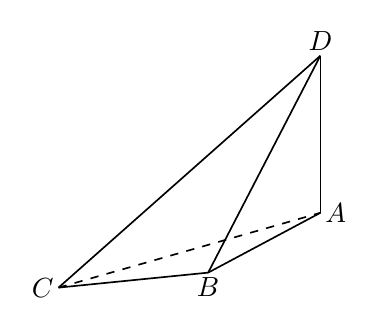
\begin{tikzpicture}[scale=0.95, semithick, every node/.style={inner sep=1.5pt}]
  \coordinate (D) at (5.0,4.7);
  \coordinate (A) at (5.0,2.6);
  \coordinate (B) at (3.5,1.8);
  \coordinate (C) at (1.5,1.6);

  \draw (D) -- (A);
  \draw (D) -- (B);
  \draw (D) -- (C);
  \draw (A) -- (B) -- (C);
  \draw[dashed] (C) -- (A);

  \node[above] at (D) {$D$};
  \node[right] at (A) {$A$};
  \node[below] at (B) {$B$};
  \node[left] at (C) {$C$};
\end{tikzpicture}
\end{center}
\nopagebreak[4]
\Needspace{4\baselineskip}
\textbf{解析}

\Needspace{5\baselineskip}
取坐标系使

\nopagebreak[4]
\[A(0,0,0),\quad B(\sqrt3,0,0),\quad C(\sqrt3,\sqrt3,0),\quad D(0,0,\sqrt3).\]

\Needspace{5\baselineskip}
$\triangle ABC$ 的外心为 $AC$ 中点 $M\left(\dfrac{\sqrt3}2,\dfrac{\sqrt3}2,0\right)$，球心 $O'\left(\dfrac{\sqrt3}2,\dfrac{\sqrt3}2,h\right)$。由 $|O'A|=|O'D|$：

\nopagebreak[4]
\[h^2+\frac32=\frac32+\left(h-\sqrt3\right)^2\ \Longrightarrow\ h=\frac{\sqrt3}2,\qquad R^2=\frac94,\qquad R=\frac32.\]

\nopagebreak[4]
\[V=\frac43\pi R^3=\frac43\pi\cdot\frac{27}8=\frac{9\pi}2.\]

\gkanswer{答案：$\dfrac{9\pi}2$。}

\end{answer}
\begin{answer}
\gksolhead{15}{}

\textbf{题目}：

已知 $t$ 为常数，函数 $y=\left|x^2-2x-t\right|$ 在区间 $[0,3]$ 上的最大值为 $2$，则 $t=$\gkblank{}。

\Needspace{4\baselineskip}
\textbf{解析}

\Needspace{5\baselineskip}
$f(x)=x^2-2x-t=(x-1)^2-1-t$ 在 $[0,3]$ 上的取值为 $f(0)=-t$，$f(1)=-1-t$，$f(3)=3-t$。故

\nopagebreak[4]
\[\max_{[0,3]}\left|x^2-2x-t\right|=\max\left\{|t|,\ |t+1|,\ |t-3|\right\}=2.\]

分区间讨论：$t\geqslant1$ 时最大值为 $|t+1|=t+1$，得 $t=1$；$0\leqslant t<1$ 时最大值为 $|t-3|=3-t=2$，得 $t=1$（不合）；$t<0$ 时最大值为 $|t-3|=3-t=2$，得 $t=1$（不合）。故 $t=1$。

\gkanswer{答案：$1$。}

\end{answer}
\begin{answer}
\gksolhead{16}{}

\textbf{题目}：

用 $1,2,3,4,5,6$ 组成六位数（没有重复数字），要求任何相邻两个数字的奇偶性不同，且 $1$ 和 $2$ 相邻，这样的六位数的个数是\gkblank{}。（用数字作答）

\Needspace{4\baselineskip}
\textbf{解析}

\Needspace{5\baselineskip}
相邻两数奇偶性不同，故只有“奇偶奇偶奇偶”“偶奇偶奇偶奇”两种模式；$1$ 占奇数位、$2$ 占偶数位，二者相邻的位置共 $5$ 对，每对只有“$1$ 在前”一种填法，余下两个奇数与两个偶数各 $2!$ 种。故

\nopagebreak[4]
\[2\times5\times2\times2=40.\]

\gkanswer{答案：$40$。}

\end{answer}
\begin{answer}
\gksolhead{17}{}

\textbf{题目}：

若 $a\geqslant0$，$b\geqslant0$，且当 $\begin{cases}x\geqslant0,\\ y\geqslant0,\\ x+y\leqslant1\end{cases}$ 时，恒有 $ax+by\leqslant1$，则以 $a$，$b$ 为坐标的点 $P(a,b)$ 所形成的平面区域的面积等于\gkblank{}。

\Needspace{4\baselineskip}
\textbf{解析}

对固定的 $a$，$b\geqslant0$，$ax+by$ 在三角形（顶点 $(0,0)$，$(1,0)$，$(0,1)$）上的最大值为 $\max\{a,b\}$，故条件等价于 $a\leqslant1$，$b\leqslant1$，区域是边长为 $1$ 的正方形，面积为 $1$。

\gkanswer{答案：$1$。}

\end{answer}
\begin{answer}
\gksolhead{18}{}

\textbf{题目}：

如图，矩形 $ABCD$ 和梯形 $BEFC$ 所在平面互相垂直，$BE\parallel CF$，$\angle BCF=\angle CEF=90^\circ$，$AD=\sqrt3$，$EF=2$。

（1）求证：$AE\parallel$ 平面 $DCF$；

（2）当 $AB$ 的长为何值时，二面角 $A-EF-C$ 的大小为 $60^\circ$？
\nopagebreak[4]
\begin{center}% 2008 年浙江卷理科第 20 题：矩形 ABCD 与梯形 BEFC 所在平面互相垂直，BE∥CF，
%   ∠BCF=∠CEF=90°，AD=√3，EF=2。
% 来源 PDF：gaokaomath-src/普通高考/2008/2008浙江理.pdf
% SHA-256：61b86d188443ba25020577365e293aa0999ec32fb32b9791690cec6ac85cf0db
% 原页：2008浙江理.pdf 第 2 页（A3 三栏）第 1 栏，书页码 492。
% 重绘依据：按斜投影作图，保持 AB∥DC、AD∥BC、BE∥CF；A 左上、B 左下、D 右上、C 居中、
%   E 在中下、F 在右下；可见棱 AB、AD、AC、AE、AF、DF、BE、EF 实线，自 C 出发的
%   BC、CD、CE、CF 被遮挡用虚线。
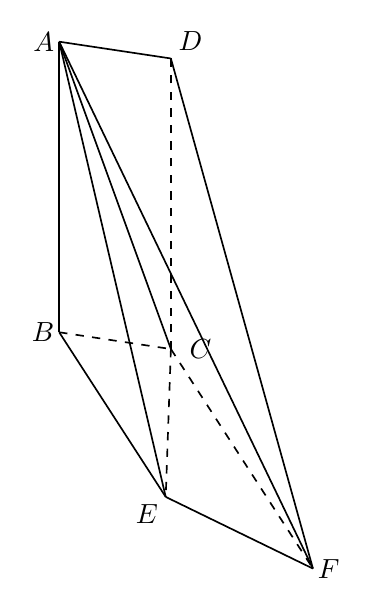
\begin{tikzpicture}[scale=0.82, semithick, every node/.style={inner sep=1.5pt}]
  \coordinate (A) at (1.00,8.50);
  \coordinate (B) at (1.00,4.00);
  \coordinate (C) at (2.73,3.74);
  \coordinate (D) at (2.73,8.24);
  \coordinate (E) at (2.65,1.45);
  \coordinate (F) at (4.93,0.34);

  % 可见棱
  \draw (A) -- (B);
  \draw (A) -- (D);
  \draw (A) -- (C);
  \draw (A) -- (E);
  \draw (A) -- (F);
  \draw (D) -- (F);
  \draw (B) -- (E);
  \draw (E) -- (F);

  % 被遮挡的棱（自 C 出发）
  \draw[dashed] (B) -- (C);
  \draw[dashed] (C) -- (D);
  \draw[dashed] (C) -- (E);
  \draw[dashed] (C) -- (F);

  \node[left] at (A) {$A$};
  \node[left] at (B) {$B$};
  \node[right=5pt] at (C) {$C$};
  \node[above right=1pt] at (D) {$D$};
  \node[below left=1pt] at (E) {$E$};
  \node[right] at (F) {$F$};
\end{tikzpicture}
\end{center}
\nopagebreak[4]
\Needspace{4\baselineskip}
\textbf{解析}

（1）取 $B$ 为原点，$BC$ 所在直线为 $y$ 轴，平面 $ABCD$ 为 $z=0$ 平面，平面 $BEFC$ 为 $x=0$ 平面。设 $AB=a$，则 $A(a,0,0)$，$D(a,\sqrt3,0)$，$C(0,\sqrt3,0)$，$E(0,0,s)$，$F(0,\sqrt3,t)$。由 $\angle CEF=90^\circ$ 与 $EF=2$ 得 $s(t-s)=3$，$(t-s)^2=1$，取 $t-s=1$，$s=3$，$t=4$。

平面 $DCF$ 过 $D$，$C$，$F$，三点 $y$ 坐标均为 $\sqrt3$，故为 $y=\sqrt3$；$\overrightarrow{AE}=(-a,0,3)$ 的 $y$ 分量为 $0$，且 $A\notin$ 平面 $DCF$，故 $AE\parallel$ 平面 $DCF$。

\Needspace{5\baselineskip}
（2）平面 $CEF$ 即 $x=0$，法向量 $\boldsymbol n_1=(1,0,0)$；平面 $AEF$ 的法向量

\nopagebreak[4]
\[\boldsymbol n_2=\overrightarrow{AE}\times\overrightarrow{AF}=\left(-3\sqrt3,\ a,\ -a\sqrt3\right),\qquad |\boldsymbol n_2|=\sqrt{27+4a^2}.\]

\Needspace{5\baselineskip}
由二面角 $60^\circ$：

\nopagebreak[4]
\[\frac{3\sqrt3}{\sqrt{27+4a^2}}=\frac12\ \Longrightarrow\ 27+4a^2=108\ \Longrightarrow\ a=\frac92.\]

\gkanswer{答案：（1）证明见解析；（2）$AB=\dfrac92$。}

\end{answer}
\begin{answer}
\gksolhead{19}{}

\textbf{题目}：

一个袋中有若干个大小相同的黑球、白球和红球。已知从袋中任意摸出 $1$ 个球，得到黑球的概率是 $\dfrac25$；从袋中任意摸出 $2$ 个球，至少得到 $1$ 个白球的概率是 $\dfrac79$。

（1）若袋中共有 $10$ 个球，

① 求白球的个数；

② 从袋中任意摸出 $3$ 个球，记得到白球的个数为 $\xi$，求随机变量 $\xi$ 的数学期望 $E\xi$。

（2）求证：从袋中任意摸出 $2$ 个球，至少得到 $1$ 个黑球的概率不大于 $\dfrac7{10}$，并指出袋中哪种颜色的球个数最少。

\Needspace{4\baselineskip}
\textbf{解析}

\Needspace{5\baselineskip}
（1）① 黑球 $10\times\dfrac25=4$ 个。设白球 $w$ 个，由

\nopagebreak[4]
\[1-\frac{\mathrm C_{10-w}^2}{\mathrm C_{10}^2}=\frac79\ \Longrightarrow\ (10-w)(9-w)=20\ \Longrightarrow\ w=5\ \text{\text{或}}\ 14,\]

由 $w\leqslant10$ 得 $w=5$。

\Needspace{5\baselineskip}
② $\xi$ 服从超几何分布（$N=10$，$K=5$，$n=3$），故

\nopagebreak[4]
\[E\xi=3\times\frac5{10}=\frac32.\]

\Needspace{5\baselineskip}
（2）设袋中共有 $N$ 个球、黑球 $b$ 个，由 $P(\text{\text{黑}})=\dfrac25$ 得 $b=\dfrac{2N}5$，故 $N$ 是 $5$ 的倍数且 $N\geqslant5$。于是 $N-b=\dfrac{3N}5$，

\nopagebreak[4]
\[P(\text{\text{至少} }1\text{ \text{个黑}})=\ 1-\frac{\mathrm C_{N-b}^2}{\mathrm C_N^2}
=1-\frac{3(3N-5)}{25(N-1)}=\frac{16N-10}{25(N-1)}.\]

\Needspace{5\baselineskip}
由 $N\geqslant5$：

\nopagebreak[4]
\[\frac{16N-10}{25(N-1)}\leqslant\frac7{10}\ \Longleftrightarrow\ 10(16N-10)\leqslant175(N-1)\ \Longleftrightarrow\ 15N\geqslant75,\]

故不等式成立。结合（1）的 $N=10$、$b=4$、$w=5$，红球 $10-4-5=1$ 个，个数最少。

\gkanswer{答案：（1）① $5$；② $\dfrac32$；（2）证明见解析，红球最少。}

\end{answer}
\begin{answer}
\gksolhead{20}{}

\textbf{题目}：

已知曲线 $C$ 是到点 $P\left(-\dfrac12,\dfrac38\right)$ 和到直线 $y=-\dfrac58$ 距离相等的点的轨迹。$l$ 是过点 $Q(-1,0)$ 的直线，$M$ 是 $C$ 上（不在 $l$ 上）的动点；$A$，$B$ 在 $l$ 上，$MA\perp l$，$MB\perp x$ 轴（如图）。

（1）求曲线 $C$ 的方程；

（2）求出直线 $l$ 的方程，使得 $\dfrac{|QB|^2}{|QA|}$ 为常数。
\nopagebreak[4]
\begin{center}% 2008 年浙江卷理科第 20 题：曲线 C 是到点 P(−1/2,3/8) 与直线 y=−5/8 距离相等的点的轨迹；
%   l 过 Q(−1,0)，M 在 C 上，A、B 在 l 上，MA⊥l，MB⊥x 轴。
% 来源 PDF：gaokaomath-src/普通高考/2008/2008浙江理.pdf
% SHA-256：61b86d188443ba25020577365e293aa0999ec32fb32b9791690cec6ac85cf0db
% 原页：2008浙江理.pdf 第 2 页（A3 三栏）第 1 栏，书页码 492。
% 重绘依据：原图为示意图，仅画坐标轴、过 Q 的直线 l、M 及其到 l 的垂足 A、到 x 轴的垂足 B，
%   曲线 C 本身不画出（与原图一致）。
\begin{tikzpicture}[scale=1.1, semithick, font=\small, every node/.style={inner sep=1.2pt}]
  \draw[->,>=stealth] (-2.6,0) -- (4.8,0) node[right] {$x$};
  \draw[->,>=stealth] (0,-1.2) -- (0,4.4) node[above] {$y$};
  \node[below left] at (0,0) {$O$};

  % 直线 l：过 Q(-1,0)，斜率 0.45
  \draw (-2.4,-0.63) -- (4.6,2.52) node[right] {$l$};
  \fill (-1,0) circle (1.2pt);
  \node[below right] at (-1,0) {$Q$};

  % M、B、A
  \coordinate (M) at (2.6,3.3);
  \coordinate (B) at (2.6,1.62);
  \coordinate (A) at (3.229,1.903);
  \draw (M) -- (B);
  \draw (M) -- (A);
  % A 处的直角标记
  \draw (3.09,1.80) -- (3.16,1.95) -- (3.32,1.86);
  \node[above left] at (M) {$M$};
  \node[below left] at (B) {$B$};
  \node[right] at (A) {$A$};
\end{tikzpicture}
\end{center}
\nopagebreak[4]
\Needspace{4\baselineskip}
\textbf{解析}

\Needspace{5\baselineskip}
（1）设 $M(x,y)$，由到 $P$ 与到直线的距离相等：

\nopagebreak[4]
\[\left(x+\frac12\right)^2+\left(y-\frac38\right)^2=\left(y+\frac58\right)^2,\]

\Needspace{5\baselineskip}
化简得

\nopagebreak[4]
\[\left(x+\frac12\right)^2=2y+\frac14,\qquad\text{\text{即} }y=\frac{x^2}2+\frac x2.\]

\Needspace{5\baselineskip}
（2）设 $l:y=k(x+1)$，$M\left(m,\dfrac{m^2}2+\dfrac m2\right)$，则 $B\left(m,k(m+1)\right)$，

\nopagebreak[4]
\[|QB|^2=(m+1)^2\left(1+k^2\right).\]

\Needspace{5\baselineskip}
$A$ 是 $M$ 在 $l$ 上的射影，$\overrightarrow{QM}=\left(m+1,\dfrac{m^2+m}2\right)$，$l$ 的单位方向向量 $\dfrac{(1,k)}{\sqrt{1+k^2}}$，故

\nopagebreak[4]
\[|QA|=\frac{\left|(m+1)+\dfrac{k\left(m^2+m\right)}2\right|}{\sqrt{1+k^2}}=\frac{|m+1|\left|1+\dfrac{km}2\right|}{\sqrt{1+k^2}}.\]

\Needspace{5\baselineskip}
于是

\nopagebreak[4]
\[\frac{|QB|^2}{|QA|}=\left(1+k^2\right)^{3/2}\cdot\frac{|m+1|}{\left|1+\dfrac{km}2\right|}.\]

\Needspace{5\baselineskip}
要与 $m$ 无关，需 $1+\dfrac{km}2$ 与 $m+1$ 成比例，即 $k=2$。此时比值为 $5\sqrt5$，故

\nopagebreak[4]
\[l:\ y=2(x+1),\qquad\text{\text{即} }2x-y+2=0.\]

\gkanswer{答案：（1）$y=\dfrac{x^2}2+\dfrac x2$；（2）$2x-y+2=0$。}

\end{answer}
\begin{answer}
\gksolhead{21}{}

\textbf{题目}：

已知 $a$ 是实数，函数 $f(x)=\sqrt x(x-a)$。

（1）求函数 $f(x)$ 的单调区间；

（2）设 $g(a)$ 为 $f(x)$ 在区间 $[0,2]$ 上的最小值。

① 写出 $g(a)$ 的表达式；

② 求 $a$ 的取值范围，使得 $-6\leqslant g(a)\leqslant-2$。

\Needspace{4\baselineskip}
\textbf{解析}

（1）定义域 $x\geqslant0$，$f'(x)=\dfrac{3x-a}{2\sqrt x}$。

当 $a\leqslant0$ 时 $f'(x)>0$，$f$ 在 $(0,+\infty)$ 上递增；当 $a>0$ 时，$f$ 在 $\left(0,\dfrac a3\right)$ 上递减，在 $\left(\dfrac a3,+\infty\right)$ 上递增。

\Needspace{5\baselineskip}
（2）① 由（1）：

\nopagebreak[4]
\[g(a)=\begin{cases}0,&a\leqslant0,\\[4pt]-\dfrac{2a^{3/2}}{3\sqrt3},&0<a\leqslant6,\\[8pt]\sqrt2(2-a),&a>6.\end{cases}\]

（其中 $a>6$ 时最小值在 $x=2$ 处取到。）

② 当 $a\leqslant0$ 时 $g(a)=0$，不合；当 $0<a\leqslant6$ 时由 $-\dfrac{2a^{3/2}}{3\sqrt3}\in[-6,-2]$ 得 $a\in[3,9]$，与 $a\leqslant6$ 取交得 $a\in[3,6]$；当 $a>6$ 时由 $\sqrt2(2-a)\in[-6,-2]$ 得 $a\in\left(6,2+3\sqrt2\right]$。

综上 $a\in\left[3,2+3\sqrt2\right]$。

\gkanswer{答案：（1）见解析；（2）① 分段表达式；② $\left[3,2+3\sqrt2\right]$。}

\end{answer}
\begin{answer}
\gksolhead{22}{}

\textbf{题目}：

已知数列 $\{a_n\}$，$a_n\geqslant0$，$a_1=0$，$a_{n+1}^2+a_{n+1}-1=a_n^2$（$n\in\mathbf N^*$）。记 $S_n=a_1+a_2+\cdots+a_n$，$T_n=\dfrac1{1+a_1}+\dfrac1{(1+a_1)(1+a_2)}+\cdots+\dfrac1{(1+a_1)(1+a_2)\cdots(1+a_n)}$。求证：当 $n\in\mathbf N^*$ 时，

（1）$a_n<a_{n+1}$；

（2）$S_n>n-2$；

（3）$T_n<3$。

\Needspace{4\baselineskip}
\textbf{解析}

（1）记 $h(x)=x^2+x$，它在 $[0,+\infty)$ 上递增，且由递推式 $h(a_{n+1})=1+a_n^2$。由 $a_n\geqslant0$ 知 $h(a_{n+1})\geqslant1>0$，故 $a_{n+1}>0$。

\Needspace{5\baselineskip}
若 $a_n<1$，则 $h(a_{n+1})=1+a_n^2<2=h(1)$，由 $h$ 递增得 $a_{n+1}<1$；又

\nopagebreak[4]
\[h(a_{n+1})-h(a_n)=\left(1+a_n^2\right)-a_n^2-a_n=1-a_n>0,\]

故 $a_{n+1}>a_n$。由 $a_1=0<1$ 归纳，对一切 $n$ 有 $a_n<1$ 且 $a_n<a_{n+1}$。

\Needspace{5\baselineskip}
（2）对 $k=1,2,\cdots,n-1$ 求和：

\nopagebreak[4]
\[\sum_{k=1}^{n-1}\left(a_{k+1}^2-a_k^2\right)+\sum_{k=1}^{n-1}a_{k+1}=n-1,\]

即 $a_n^2+S_n=n-1$，故 $S_n=n-1-a_n^2>n-2$（因 $a_n<1$）。

\Needspace{5\baselineskip}
（3）由 $a_1=0$ 得 $a_2^2+a_2-1=0$，$a_2=\dfrac{\sqrt5-1}2>\dfrac12$，结合（1）知 $a_k>\dfrac12$（$k\geqslant2$），故 $1+a_k>\dfrac32$（$k\geqslant2$）。

\nopagebreak[4]
\[T_n=1+\sum_{k=2}^n\frac1{(1+a_1)(1+a_2)\cdots(1+a_k)}
<1+\frac1{1+a_2}\sum_{j=0}^{n-2}\left(\frac23\right)^j
<1+\frac1{1+a_2}\cdot3.\]

\Needspace{5\baselineskip}
由 $1+a_2=\dfrac{1+\sqrt5}2>1.6>\dfrac43$ 得

\nopagebreak[4]
\[T_n<1+\frac{3}{1.6}<1+2=3.\qquad\blacksquare\]

\gkanswer{答案：（1）（2）（3）证明见解析。}

\end{answer}